\chapter{Desarrollo}

\section{Introducción}

El desarrollo del proyecto se ha estructurado en múltiples fases secuenciales, cada una diseñada para abordar aspectos específicos del proceso de análisis hiperespectral aplicado a la detección de aflatoxinas en higos frescos. La metodología desarrollada implementa técnicas de visión por computador de última generación combinadas con procesamiento especializado de datos hiperespectrales para crear un sistema automatizado de análisis de muestras.

\section{Entorno de Desarrollo}

El proyecto se ha implementado utilizando un entorno de desarrollo adaptado para procesamiento de imágenes hiperespectrales y ejecución de modelos de aprendizaje profundo. A continuación se detallan los aspectos fundamentales de la infraestructura técnica utilizada.

\subsection{Gestión de Entornos y Dependencias}

El proyecto se desarrolló utilizando el lenguaje de programación \emph{Python} \cite{van1995python} en su versión 3.13 con soporte para \emph{Cython} \cite{behnel2011cython}, lo que proporcionó ventajas significativas en términos de rendimiento.

\vspace{5mm}

Para la gestión de entornos virtuales se utilizó \emph{Conda} \cite{anaconda}, un sistema que permite crear espacios de trabajo aislados con versiones específicas de bibliotecas.
\vspace{5mm}

Sobre la base de \emph{Conda}, se implementó \emph{UV} \cite{uv2024github}, un gestor de paquetes y proyectos para \emph{Python}, extremadamente rápido y escrito en \emph{Rust} \cite{matsakis2014rust}. \emph{UV} fue utilizado para la instalación y gestión de paquetes dentro del entorno \emph{Conda}, aprovechando su capacidad para resolver dependencias de manera más eficiente y rápida que las herramientas tradicionales como \emph{pip} o el propio instalador de \emph{Conda}. Esta combinación permitió mantener un entorno consistente y reproducible mientras se optimizaba el tiempo de instalación y actualización de dependencias.

\vspace{5mm}

Para cada fase del proyecto se creó un paquete independiente con dependencias específicas según los requisitos de cada etapa. Las principales bibliotecas utilizadas en el proyecto incluyen:

\begin{itemize}
    \item \textbf{PyTorch con torchvision y torchaudio}: Framework principal para implementación de modelos de aprendizaje profundo \cite{NEURIPS2019_9015}. 
    \item \textbf{NumPy y SciPy}: Para operaciones numéricas y manipulación eficiente de matrices \cite{2020NumPy-Array, 2020SciPy-NMeth}.
    \item \textbf{Scikit-learn}: Para implementación de algoritmos de aprendizaje automático y métricas \cite{sklearn_api}.
    \item \textbf{Spectral}: Biblioteca especializada para procesamiento de imágenes hiperespectrales \cite{thomas_boggs_2022_7135091}.
    \item \textbf{OpenCV-Python}: Para operaciones de procesamiento de imágenes y visión por computador \cite{opencv_library}.
    \item \textbf{Transformers}: Para implementación y uso de modelos basados en arquitecturas de \emph{transformers} \cite{wolf-etal-2020-transformers}.
    \item \textbf{Timm}: Colección de modelos preentrenados para tareas de visión por computador \cite{rw2019timm}.
    \item \textbf{Supervision}: Para visualización y análisis de resultados de detección y segmentación \cite{Roboflow_Supervision}.
    \item \textbf{PyCocoTools}: Para manipulación de anotaciones en formato \emph{COCO} \cite{Welsh2018,Hoops2006,Medley2018}.
    \item \textbf{DEAP}: Para implementación de algoritmos genéticos y evolutivos \cite{DEAP_JMLR2012}.
\end{itemize}

\sloppy
Adicionalmente, se incorporaron bibliotecas auxiliares como \texttt{addict}, \texttt{colorlog}, \texttt{gdown}, \texttt{split-folders}, \texttt{submitit} y \texttt{termcolor} para tareas de gestión de configuración, logging, descarga de modelos pre-entrenados, organización de datos y paralelización de tareas.

\vspace{5mm}

La gestión precisa de versiones de estas dependencias resultó crítica para garantizar la compatibilidad entre componentes y estabilidad del entorno de desarrollo.

\subsection{Entorno de Desarrollo Integrado}

Para el desarrollo del código se empleó Visual Studio Code (VS Code) como entorno de desarrollo integrado.

\subsection{Infraestructura Computacional}

El desarrollo y ejecución del proyecto se realizó en un servidor de alto rendimiento proporcionado por la Universidad de Extremadura, con las siguientes especificaciones técnicas:

\begin{itemize}
    \item \textbf{Procesador}:  Intel(R) Xeon(R) Silver 4310 CPU @ 2.10GHz.
    \item \textbf{Memoria RAM}: 512 GB DDR4.
    \item \textbf{Acelerador Gráfico}: 4 × NVIDIA A100 con 40 GB de memoria VRAM cada una, de las cuales se utilizó una para la ejecución de los modelos de aprendizaje profundo.
    \item \textbf{Almacenamiento}: 4 TB en disco SSD NVMe.
\end{itemize}

\subsection{Adquisición de Imágenes Hiperespectrales}

Las imágenes fueron capturadas utilizando una cámara hiperespectral \emph{SPECIM}, específicamente el modelo \emph{FX10 VNIR}, cuyas características técnicas principales incluyen: resolución espacial de 1024 píxeles (800 ancho × 1024 alto), rango espectral de 400 nm a 1000 nm (visible y parte del infrarrojo cercano), 448 bandas espectrales, y un salto espectral de 1.339 nm.

\vspace{5mm}

El conjunto de datos comprende 320 higos cosechados de la plantación de la variedad calabacita ubicada en la \emph{Finca La Orden-Valdesequera} (38°51' N, 6°40' W, altitud 184 m) en Guadajira, España, donde \emph{CICYTEX} tiene su sede central. Las imágenes hiperespectrales se capturaron durante un período de 2 semanas, utilizando cada semana 160 higos cosechados en diferentes etapas de madurez.

\vspace{5mm}

Cada semana, 160 higos se dividieron en cuatro subconjuntos de aproximandamente 40 especímenes cada uno. El primer grupo correspondió a los controles sanos (Clase 0), mientras que los tres grupos siguientes fueron inoculados con concentraciones de $10^3$ UFC/mL (Clase 1), $10^5$ UFC/mL (Clase 2), y $10^7$ UFC/mL (Clase 3), respectivamente. El proceso de inoculación se realizó mediante inmersión del área durante aproximadamente 3 segundos, siguiendo el protocolo establecido por \emph{CICYTEX}.

\vspace{5mm}

Las imágenes hiperespectrales se capturaron después de la inoculación cada 24 horas durante cinco días consecutivos. Entre cada sesión de adquisición, las muestras se almacenaron en una cámara de incubación controlada a 25°C, con humedad relativa entre 80 y 90\% para promover el crecimiento fúngico. Cada clase consistió de 380 imágenes hiperespectrales, generando un total de 1520 imágenes hiperespectrales para el conjunto de datos completo.

\vspace{5mm}

Las imágenes hiperespectrales capturadas se almacenan en una estructura de directorios organizada que incluye múltiples archivos asociados a cada adquisición. A continuación, se describe el formato y contenido de los archivos principales:

\begin{itemize}
    \item \textbf{Archivos de datos hiperespectrales (\texttt{.hdr}, \texttt{.raw})}: 
    \begin{itemize}
        \item El archivo \texttt{.hdr} contiene metadatos descriptivos de la imagen, como dimensiones espaciales, número de bandas espectrales, rango espectral, y formato de datos.
        \item El archivo \texttt{.raw} almacena los datos espectrales en bruto, organizados en un formato binario que representa la intensidad de cada banda para cada píxel.
    \end{itemize}
    \item \textbf{Referencias de calibración (\texttt{DARKREF}, \texttt{WHITEREF})}: 
    \begin{itemize}
        \item Los archivos \texttt{DARKREF} y \texttt{WHITEREF} contienen las referencias oscura y blanca necesarias para la posterior corrección radiométrica de las imágenes hiperespectrales.
    \end{itemize}
    \item \textbf{Imagen \texttt{.png}}: 
    \begin{itemize}
        \item Este archivo representa una visualización en falso color \emph{RGB} generada a partir de tres bandas seleccionadas del cubo hiperespectral.
    \end{itemize}
    \item \textbf{Archivos de metadatos (\texttt{.xml})}: 
    \begin{itemize}
        \item Contienen información adicional sobre las condiciones de captura, como fecha, hora, y parámetros experimentales.
    \end{itemize}
\end{itemize}

Esta estructura permite un manejo eficiente de los datos, facilitando tanto la corrección radiométrica como la integración con el flujo de procesamiento automatizado.


\section{Localización y Segmentación de Figuras}

\subsection{Objetivo de la Fase}
La primera fase del proyecto consiste en la creación del conjunto de datos mediante la localización y segmentación automatizada de higos individuales sobre las imágenes creadas a través del falso color \emph{RGB}. El objetivo principal es generar anotaciones precisas en formato COCO \cite{lin2015microsoftcococommonobjects}, que incluyan cuadros delimitadores y máscaras de segmentación para cada higo detectado, y extraer los subcubos hiperespectrales radiométricamente corregidos correspondientes a cada fruto.

\vspace{5mm}

Esta fase es fundamental para el flujo de trabajo completo, ya que permite el aislamiento automatizado de las regiones de interés que servirán como imágenes de entrada para el entrenamiento y la inferencia de la \emph{CNN}. La precisión en esta etapa condiciona directamente la calidad de los datos que utilizará la red en las fases posteriores, por lo que resulta esencial garantizar su exactitud.

\subsection{Herramientas y Tecnologías Empleadas}

La implementación de esta fase se basa en la integración de modelos de visión por computador de última generación, complementados con librerías especializadas para el procesamiento de datos hiperespectrales y manipulación de anotaciones.

\subsubsection{Grounding DINO}

\emph{Grounding DINO} \cite{liu2023grounding,ren2024grounding} es un modelo de inteligencia artificial de última generación especializado en la detección de objetos en imágenes mediante el uso combinado de descripciones textuales e información visual, permitiendo un análisis multimodal avanzado. Gracias a su arquitectura basada en \emph{transformers} \cite{vaswani2023attentionneed} y técnicas de aprendizaje profundo, puede localizar y etiquetar objetos de interés, sin necesidad de entrenamiento específico para cada tipo de objeto, lo que lo hace altamente adaptable para tareas de detección abiertas o \emph{zero-shot} \cite{socher2013zeroshotlearningcrossmodaltransfer}.

\subsubsection{SAM2 (Segment Anything Model 2)}

\emph{SAM (Segment Anything Model)} \cite{kirillov2023segany, ravi2024sam2segmentimages} es un modelo de inteligencia artificial de última generación diseñado para segmentar cualquier objeto en imágenes o videos de manera automática y versátil. Fue desarrollado por \emph{Meta AI} y su objetivo principal es permitir la segmentación de objetos de imágenes y videos sin necesidad de entrenamiento específico para cada clase, usando tecnologías de visión por computador avanzadas y aprendizaje \emph{zero-shot}. Está entrenado en uno de los mayores conjuntos de datos existentes (SA-1B), con 11 millones de imágenes y 1.1 mil millones de máscaras de segmentación, lo que le da una capacidad sobresaliente para generalizar a nuevos contextos visuales.

\subsubsection{COCO (Common Objects in Context)}
El formato COCO (Common Objects in Context) \cite{lin2015microsoftcococommonobjects} es un estándar ampliamente adoptado para el almacenamiento y intercambio de anotaciones en tareas de visión por computador, especialmente en detección de objetos, segmentación de instancias y estimación de poses. Desarrollado por \emph{Microsoft Research},  \emph{COCO} define una estructura \emph{JSON} \cite{crockford2006application} que organiza metadatos de imágenes, anotaciones de objetos y categorías de manera eficiente y escalable.

\vspace{5mm}

Entre las componentes que definen la estructura del formato \emph{COCO}, se encuentran las \textbf{anotaciones (\emph{annotations})}, las cuales contienen las anotaciones específicas de cada objeto detectado, incluyendo identificadores únicos, referencias a imagen y categoría, coordenadas de bounding box, área, máscaras de segmentación en formato \emph{RLE (Run-Length Encoding)}, y banderas adicionales como \emph{iscrowd}, que indica si el objeto es parte de un grupo denso.

\vspace{5mm}

Para tareas de segmentación de instancias, las máscaras se codifican mediante \emph{RLE}, un algoritmo de compresión sin pérdidas que representa secuencias de píxeles consecutivos como pares (valor, longitud), reduciendo significativamente el espacio de almacenamiento requerido. Las coordenadas de bounding box se especifican en formato \texttt{[x, y, width, height]}, donde \texttt{(x, y)} representa la esquina superior izquierda del rectángulo delimitador.


\subsection{Flujo de Procesamiento}

La implementación del flujo de trabajo se diseñó siguiendo una arquitectura modular que separa conceptualmente la detección y anotación automatizada de la extracción de subcubos hiperespectrales. Esta separación se materializa en dos módulos principales: el primero responsable de la localización y segmentación de higos individuales sobre las imágenes RGB derivadas, y el segundo encargado de la extracción de los subcubos hiperespectrales correspondientes a cada detección validada.

\vspace{5mm}

El sistema adopta un patrón de procesamiento por lotes que opera sistemáticamente sobre la estructura jerárquica del conjunto de datos. Cada directorio de clase (C0, C1, C2, C3) contiene las imágenes hiperespectrales junto con sus archivos de metadatos y referencias de calibración.

\subsubsection{1. Detección}

El módulo de detección y segmentación constituye el núcleo del flujo automatizado. La implementación utiliza \emph{Grounding DINO} como modelo de detección, empleando la arquitectura con la red principal (\emph{backbone}) \emph{Swin Transformer Base} y el punto de control preentrenado correspondiente. Esta configuración permite al modelo procesar imágenes \emph{RGB} manteniendo su relación de aspecto original mientras utiliza la entrada de  texto \emph{fig} (higo en inglés) como descriptor semántico para guiar la detección.

\vspace{5mm}

La optimización de los parámetros de inferencia se estableció mediante experimentación empírica, fijando tanto el umbral de confianza de detección como el umbral de similaridad semántica texto-imagen en 0.25. Esta configuración proporciona un equilibrio óptimo entre sensibilidad de detección y precisión para el conjunto de datos específico, minimizando tanto los falsos positivos como los falsos negativos. El proceso de detección implementa una secuencia de validación que comienza con la carga de imágenes seguida de la conversión del espacio de color \emph{BGR} a \emph{RGB} y la extracción automática de metadatos temporales y experimentales del nombre del archivo.

\vspace{5mm}

Durante la inferencia, el modelo transforma las imágenes a tensores \emph{PyTorch} aplicando la normalización correspondiente a los parámetros del modelo preentrenado, ejecuta la detección con la entrada de texto especificada y aplica un filtrado geométrico crítico que limita las dimensiones máximas de los cuadros delimitadores a 250×150 píxeles. Esta restricción dimensional resulta fundamental para asegurar la detección de higos individuales y evitar regiones que abarquen múltiples especímenes, un problema recurrente en imágenes con alta densidad de objetos. El post-procesamiento convierte las coordenadas al formato requerido por \emph{SAM-2} y extrae las puntuaciones de confianza asociadas a cada detección.

\subsubsection{2. Segmentación}

La segmentación se realiza mediante \emph{SAM-2}, inicializado con la configuración \emph{Hiera Large} y el punto de control preentrenado correspondiente, utilizando el predictor específicamente diseñado para el procesamiento de imágenes estáticas. El modelo opera sin supervisión de puntos, empleando exclusivamente los cuadros delimitadores generados por \emph{Grounding DINO} como entrada primaria. La configuración para una única máscara por detección asegura la generación coherente, simplificando el procesamiento posterior y manteniendo la consistencia en las anotaciones. La figura \ref{fig:dino_sam} muestra un ejemplo representativo del proceso de detección y segmentación automatizada implementado.

\begin{figure}[ht]
\centering
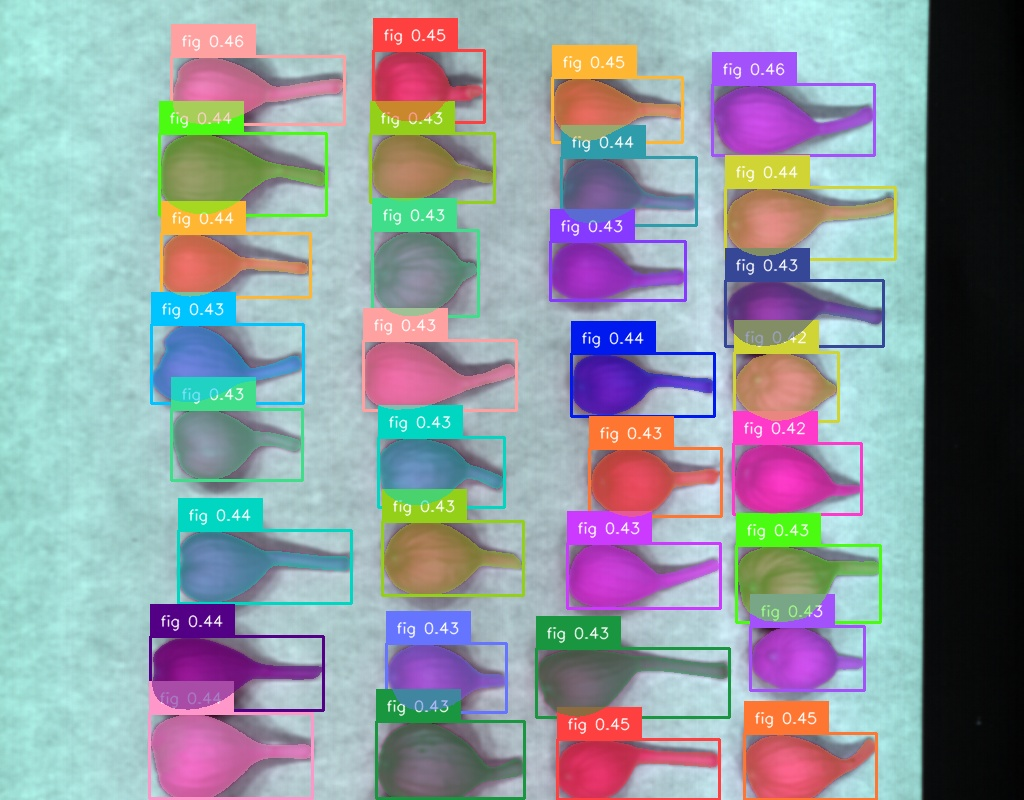
\includegraphics[width=\textwidth]{images/dino_sam.jpg}
\caption{Ejemplo de detección y segmentación de higos utilizando \emph{Grounding DINO} y \emph{SAM-2}. La imagen muestra las cajas delimitadoras generadas por \emph{Grounding DINO} y las máscaras de segmentación producidas por \emph{SAM-2}.}
\label{fig:dino_sam}
\end{figure}

\subsubsection{3. Generación de Anotaciones}

La generación de anotaciones en formato \emph{COCO} se realizó mediante la construcción sistemática de estructuras de datos que incluyen metadatos de imagen, información de categorías y listas de anotaciones. Cada máscara binaria generada por \emph{SAM-2} se transforma al formato \emph{RLE} mediante las herramientas correspondientes, calculando automáticamente el área de cada instancia y asignando identificadores únicos secuenciales. El sistema exporta los resultados como archivos \emph{JSON} organizados por clase experimental, manteniendo la trazabilidad completa desde las imágenes originales hasta las anotaciones finales.

\subsubsection{4. Extracción de Subcubos Hiperespectrales}

El último componente del flujo se encarga de la extracción de sub-cubos hiperespectrales radiométricamente corregidos a partir de las detecciones validadas en la fase anterior. Este módulo implementa un procesamiento sofisticado que combina corrección radiométrica, mapeo geométrico y extracción volumétrica para generar datos hiperespectrales de alta calidad correspondientes a cada higo individual detectado.

\begin{figure}[ht]
\centering
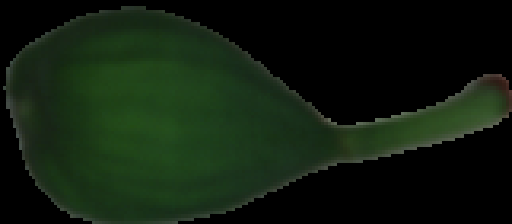
\includegraphics[width=\textwidth]{images/higo_individual_220_113_78.png}
\caption{Ejemplo de la representación en falso color \emph{RGB} de un higo individual extraído del cubo hiperespectral. Las bandas espectrales utilizadas para la visualización son 220 (Rojo), 113 (Verde) y 78 (Azul).}
\label{fig:higo_individual}
\end{figure}


\vspace{5mm}

La corrección radiométrica constituye un paso crítico para garantizar la calidad de los datos hiperespectrales, eliminando efectos de iluminación y variaciones instrumentales que podrían comprometer el análisis posterior. El proceso utiliza las referencias oscura y blanca capturadas simultáneamente con cada imagen hiperespectral, aplicando la ecuación estándar de corrección:

\begin{equation}
R = \frac{RAW - DARK}{WHITE - DARK}
\end{equation}

donde $R$ representa la reflectancia corregida, $RAW$ los datos espectrales en bruto, $DARK$ la referencia oscura y $WHITE$ la referencia blanca. La implementación incluye el tratamiento robusto de casos especiales, como la prevención de divisiones por cero en regiones donde las referencias oscura y blanca presentan valores idénticos, situación que puede ocurrir en áreas de muy baja reflectancia.

\vspace{5mm}

La extracción geométrica de sub-cubos requiere una transformación precisa desde el espacio de coordenadas \emph{RGB}, donde se realizaron las detecciones, al espacio hiperespectral correspondiente. Esta conversión considera las posibles diferencias en resolución espacial entre las imágenes \emph{RGB} derivadas y los cubos hiperespectrales originales, implementando técnicas de mapeo que preservan la correspondencia espacial exacta. El sistema valida geométricamente cada región de interés para asegurar que los subcubos extraídos no excedan los límites físicos del cubo hiperespectral, evitando errores de indexación y garantizando la integridad de los datos espectrales.

\vspace{5mm}

El proceso de extracción volumétrica utiliza técnicas de división tridimensional optimizadas para mantener la estructura espectral completa de cada región de interés. Los subcubos resultantes preservan las 448 bandas espectrales originales junto con la resolución espacial correspondiente a cada detección, manteniendo la información espectral íntegra necesaria para el análisis posterior. La organización del almacenamiento sigue una estructura jerárquica específica, con subdirectorios organizados por clase experimental (\texttt{C0}, \texttt{C1}, \texttt{C2}, \texttt{C3}). Cada subcubo se almacena en formato \texttt{.npy} de \emph{NumPy} siguiendo una nomenclatura sistemática que incluye clase, timestamp y número de instancia, facilitando tanto el acceso eficiente como la trazabilidad completa mientras preserva la precisión numérica de punto flotante y optimiza los tiempos de carga durante el entrenamiento de modelos.

\subsection{Resultados}

La ejecución completa de la primera fase genera un conjunto estructurado de elementos que constituyen la base fundamental para las fases posteriores del proyecto. Las anotaciones \emph{COCO} resultantes comprenden archivos \emph{JSON} organizados por clase experimental, cada uno conteniendo metadatos completos de detección que incluyen coordenadas de cuadros delimitadores, máscaras de segmentación en formato \emph{RLE} y metadatos temporales extraídos automáticamente del sistema de nomenclatura implementado. Esta organización sistemática permite mantener la trazabilidad completa desde las imágenes originales hasta las detecciones finales, facilitando tanto la validación manual como el procesamiento automatizado en etapas subsecuentes.

\begin{figure}[H]
\centering
\small
\begin{verbatim}
{
    "info": {
        "description": "Fig detection and segmentation dataset",
        "version": "1.0",
        "year": 2024,
        "contributor": "Hyperspectral Analysis Pipeline",
        "date_created": "2024-01-15"
    },
    "licenses": [],
    "images": [
        {
            "id": 1,
            "width": 800,
            "height": 1024,
            "file_name": "C0_2023-07-17_10-15-30_001.png",
            "date_captured": "2023-07-17T10:15:30"
        }
    ],
    "annotations": [
        {
            "id": 1,
            "image_id": 1,
            "category_id": 1,
            "segmentation": {
                "size": [1024, 800],
                "counts": "nXh04M3M2N2N1O1O1N2N2N1O1O1N2N..."
            },
            "area": 12485,
            "bbox": [245.3, 412.7, 128.4, 97.2],
            "iscrowd": 0
        }
    ],
    "categories": [
        {
            "id": 1,
            "name": "fig",
            "supercategory": "fruit"
        }
    ]
}
\end{verbatim}
\caption{Ejemplo de anotación en formato COCO para la clase 0.}
\end{figure}

\subsection{Desafíos y Observaciones Técnicas}

Durante la implementación, se identificaron y resolvieron varios desafíos técnicos que proporcionaron valiosas lecciones para el desarrollo del proyecto. El primer y más significativo desafío encontrado fue determinar las versiones correctas de \emph{PyTorch} y sus dependencias relacionadas (\emph{torchvision} y \emph{torchaudio}) que fueran compatibles tanto con \emph{Grounding DINO} como con \emph{SAM-2}. Ambos modelos requieren versiones específicas del framework que no siempre coinciden, especialmente considerando las actualizaciones frecuentes en el ecosistema de aprendizaje profundo. La solución final involucró el análisis detallado de los requisitos de compatibilidad de cada modelo y la identificación de una versión común de \emph{PyTorch} 2.1.2 con soporte \emph{CUDA} 11.8 que proporcionara estabilidad y rendimiento óptimo para ambos componentes.

\vspace{5mm}

La optimización de la memoria de la \emph{GPU} constituyó otro reto importante, dado que el procesamiento conjunto de \emph{Grounding DINO} y \emph{SAM-2} requirió una implementación cuidadosa de contextos autocast para prevenir desbordamientos de memoria. La solución implementada aplica precisión mixta de forma selectiva \cite{micikevicius2018mixedprecisiontraining}: utiliza \texttt{torch.autocast} con \texttt{dtype=torch.bfloat16} únicamente para \emph{SAM-2}, mientras mantiene precisión completa para \emph{Grounding DINO}, equilibrando eficiencia computacional con calidad de inferencia. La elección del formato \texttt{bfloat16} se fundamenta en su diseño específico para aplicaciones de aprendizaje profundo, proporcionando un rango dinámico superior a \texttt{float16} tradicional \cite{8877411}. Adicionalmente, se configuró el uso de \emph{TF32} cuando está disponible en hardware compatible para optimizar las operaciones de multiplicación de matrices.

\section{Selección de Bandas}

\subsection{Objetivo de la Fase}
La segunda fase del proyecto se centra en la optimización de la selección de bandas espectrales mediante la implementación de un algoritmo genético que identifica automáticamente las tres bandas más informativas del cubo hiperespectral. El objetivo principal es reducir la dimensionalidad de los datos hiperespectrales de manera inteligente, preservando la información espectral crítica para la clasificación de contaminación por aflatoxinas mientras se optimiza la eficiencia computacional del entrenamiento de redes neuronales.

\vspace{5mm}

La reducción de 448 bandas espectrales a una combinación RGB de tres bandas estratégicamente seleccionadas permite aprovechar arquitecturas de CNN preentrenadas diseñadas para imágenes RGB convencionales, facilitando el uso de técnicas de aprendizaje por transferencia mediante ajuste fino selectivo \cite{NEURIPS2019_9015} con modelos robustos como \emph{ResNet-50} \cite{he2016deep} sin sacrificar la capacidad discriminativa del sistema.

\subsection{Herramientas y Tecnologías Empleadas}

La implementación de esta fase integra algoritmos evolutivos de optimización con técnicas de aprendizaje profundo, creando un sistema híbrido que combina la exploración global de los algoritmos genéticos con la capacidad de generalización de las redes neuronales convolucionales.

\subsubsection{DEAP (Distributed Evolutionary Algorithms in Python)}

\emph{DEAP} \cite{DEAP_JMLR2012} es un framework innovador de computación evolutiva diseñado específicamente para el prototipado rápido y la evaluación eficiente de ideas en el ámbito de la optimización bio-inspirada. A diferencia de otros frameworks tradicionales que imponen limitaciones mediante tipos predefinidos, \emph{DEAP} adopta una filosofía de diseño que prioriza la flexibilidad y la transparencia, permitiendo a los desarrolladores crear tipos de datos apropiados, personalizar inicializadores según sus necesidades específicas y seleccionar operadores de manera explícita y fundamentada.

\vspace{5mm}

En el contexto específico de este proyecto, \emph{DEAP} facilita la implementación de un algoritmo genético especializado para la selección de bandas hiperespectrales mediante la creación de tipos personalizados que representan combinaciones de índices espectrales, operadores de cruce y mutación que respetan las restricciones del dominio (rango [0, 447]), y estrategias de selección por torneo optimizadas para el problema de clasificación.

\subsubsection{ResNet-50}

ResNet-50 \cite{he2015deepresiduallearningimage} constituye la arquitectura base empleada para evaluar la aptitud de cada individuo en el algoritmo genético. Esta red neuronal convolucional profunda introduce el concepto de \emph{residual connections}, que permiten entrenar de forma estable modelos sustancialmente más profundos al mitigar problemas de desvanecimiento del gradiente. Con sus 50 capas, \emph{ResNet-50} logra un equilibrio entre profundidad y eficiencia computacional, ofreciendo un rendimiento robusto en tareas de clasificación de imágenes. Al estar preentrenada en el extenso conjunto de datos ImageNet \cite{deng2009imagenet}, proporciona un punto de partida sólido para el aprendizaje por transferencia, lo que permite aprovechar representaciones visuales generales y adaptarlas a la tarea específica de clasificación de imágenes \emph{RGB} derivadas de las combinaciones de bandas espectrales seleccionadas por el algoritmo evolutivo.

\subsection{Flujo de Procesamiento}

El algoritmo genético implementado utiliza una arquitectura evolutiva estándar, adaptada específicamente para abordar el problema de selección de bandas hiperespectrales. Cada iteración del proceso evolutivo integra una evaluación basada en aprendizaje profundo, optimizando así la selección de bandas de manera eficiente.

\subsubsection{1. Representación y Inicialización}

Cada individuo en la población se representa mediante un vector de tres enteros en el rango [0, 447], donde cada posición del vector corresponde a una banda espectral específica: el primer entero representa la banda asignada al canal \emph{R} (rojo), el segundo entero al canal \emph{G} (verde), y el tercer entero al canal \emph{B} (azul). Estas bandas seleccionadas se combinan para formar la imagen \emph{RGB}. La población inicial se genera aleatoriamente con un tamaño de 20 individuos, valor determinado mediante experimentación empírica para equilibrar diversidad poblacional con eficiencia computacional. La inicialización uniforme garantiza la exploración inicial del espacio completo de 448 bandas disponibles, evitando sesgos hacia regiones específicas del espectro electromagnético.

\subsubsection{2. Función de Evaluación}

La evaluación de la aptitud constituye el componente más computacionalmente intensivo del algoritmo, requiriendo el entrenamiento mediante ajuste fino parcial de una red \emph{ResNet-50} para cada individuo evaluado. El proceso comienza con la construcción de imágenes \emph{RGB} utilizando las tres bandas especificadas por el individuo, seguido de la creación de cargadores de datos de \emph{PyTorch} para los conjuntos de entrenamiento y prueba.

\vspace{5mm}

El modelo \emph{ResNet-50} preentrenado en \emph{ImageNet} se adapta específicamente para el problema de clasificación de cuatro clases mediante una estrategia de aprendizaje por transferencia basada en ajuste fino selectivo. La arquitectura implementa las siguientes modificaciones: (1) congelación de todas las capas desde la entrada hasta \texttt{layer3} (inclusive), manteniendo los pesos preentrenados para la extracción de características de bajo y medio nivel; (2) liberación de los parámetros de \texttt{layer4}, la capa convolucional más profunda, permitiendo la adaptación de características de alto nivel específicas para la clasificación de higos con diferentes niveles de contaminación; y (3) reemplazo completo de la capa de clasificación final (\texttt{fc}) por una nueva capa lineal con 4 unidades de salida correspondientes a las clases \emph{C0}, \emph{C1}, \emph{C2} y \emph{C3}, inicializada aleatoriamente.

\vspace{5mm}

Esta configuración resulta en un modelo con aproximadamente 2.3 millones de parámetros entrenables de los 25.6 millones totales, concentrando el aprendizaje en las representaciones más específicas del dominio mientras preserva las características generales aprendidas en \emph{ImageNet}. El entrenamiento se ejecuta durante 50 épocas utilizando el optimizador \emph{Adam} con una tasa de aprendizaje de 0.001, aplicando técnicas de aumento de datos que incluyen volteos horizontales y verticales aleatorios, rotaciones de hasta 15 grados, y normalización estándar de \emph{ImageNet}. La aptitud final del individuo se define como la precisión de prueba alcanzada en la última época, proporcionando una medida directa de la capacidad clasificatoria de la combinación de bandas espectrales seleccionada.

\vspace{5mm}

Para optimizar la eficiencia computacional, se implementó un sistema de caché que almacena los resultados de evaluaciones previas, evitando el reentrenamiento de combinaciones de bandas ya evaluadas en generaciones anteriores.

\subsubsection{3. Operadores Genéticos}

El algoritmo implementa operadores genéticos especializados que respetan las restricciones del dominio espectral y aprovechan las características intrínsecas de la información hiperespectral. La selección de estos operadores se fundamenta en el principio de que la información espectral relevante para la clasificación tiende a concentrarse en bandas espectralmente adyacentes debido a la correlación espacial natural entre longitudes de onda vecinas en el espectro electromagnético.

\vspace{5mm}

\textbf{Operador de Cruce:} El cruce utiliza una variante modificada del operador de mezcla (\emph{blend crossover}) que combina linealmente los valores de los padres. La fórmula utilizada es:

\begin{equation}
hijo_i = (1-\gamma) \cdot padre1_i + \gamma \cdot padre2_i
\end{equation}

donde $\gamma$ se genera aleatoriamente en cada posición. Este operador resulta particularmente apropiado para la selección de bandas hiperespectrales porque produce descendientes cuyos índices de banda se mantienen en regiones espectrales intermedias entre los padres, preservando la localidad espectral y evitando saltos abruptos hacia bandas distantes que podrían no contener información correlacionada. Tras la aplicación del operador, se aplican restricciones de dominio para garantizar que los descendientes mantengan índices válidos en el rango [0, 447].

\vspace{5mm}

\textbf{Operador de Mutación:} La mutación emplea un operador gaussiano con desviación estándar de 1.0 y probabilidad individual de 0.1, seguido de restricción al dominio válido. La elección de la mutación gaussiana con desviación estándar reducida ($\sigma=1.0$) está específicamente diseñada para introducir variaciones locales que exploren bandas espectralmente cercanas a las actuales, aprovechando el hecho de que bandas adyacentes en el espectro electromagnético típicamente contienen información complementaria y correlacionada. Esta estrategia de mutación conservativa evita perturbaciones drásticas que podrían llevar la búsqueda hacia regiones espectrales completamente diferentes y potencialmente menos informativas, manteniendo la continuidad espectral mientras permite la exploración gradual del espacio de soluciones.

\vspace{5mm}

\textbf{Selección y Elitismo:} La selección de padres utiliza torneos de tamaño 3, proporcionando una presión selectiva moderada que equilibra la explotación de buenas soluciones con la exploración de nuevas regiones del espacio de búsqueda. Se implementa elitismo con tamaño 1, garantizando la preservación de la mejor solución encontrada a través de las generaciones y asegurando que el algoritmo no pierda combinaciones de bandas de alta aptitud durante el proceso evolutivo.

\subsubsection{4. Configuración Experimental}

El algoritmo se configura para ejecutar durante 50 generaciones con una población de 20 individuos, utilizando probabilidades de cruzamiento y mutación de 0.8 y 0.15 respectivamente. Estos parámetros se determinaron mediante experimentación previa para optimizar el balance entre exploración y explotación en el contexto específico del problema de selección de bandas.

\vspace{5mm}

Para garantizar la reproducibilidad y robustez estadística, se implementó un sistema de experimentos múltiples que permite la ejecución de varias corridas independientes del algoritmo, cada una con semillas aleatorias diferentes. Los resultados de cada experimento se almacenan automáticamente en archivos CSV que incluyen estadísticas generacionales completas y métricas detalladas del mejor individuo.

\subsection{Resultados}

Se realizaron diez experimentos independientes.

\begin{table}[ht]
\centering
\caption{Resumen de métricas de los experimentos de selección de bandas.}
\label{tab:experiment_metrics}
\resizebox{\textwidth}{!}{
\csvautotabular{tables/experiment_metrics_summary.csv}
}
\end{table}

\begin{table}[ht]
\centering
\caption{Resultados del experimento 10 con las bandas seleccionadas 220, 113 y 78.}
\label{tab:exp_10_cnn_results_220_113_78}
\resizebox{\textwidth}{!}{
\csvautotabular{tables/exp_10_cnn_results_220_113_78.csv}
}
\end{table}

\begin{table}[ht]
\centering
\caption{Matriz de confusión del experimento 10 con las bandas seleccionadas 220, 113 y 78.}
\label{tab:exp_10_confusion_matrix_220_113_78}
\resizebox{\textwidth}{!}{
\csvautotabular{tables/exp_10_confusion_matrix_220_113_78.csv}
}
\end{table}

\begin{table}[ht]
\centering
\caption{Reporte de clasificación del experimento 10 con las bandas seleccionadas 220, 113 y 78.}
\label{tab:exp_10_classification_report_220_113_78}
\resizebox{\textwidth}{!}{
\csvautotabular{tables/exp_10_classification_report_220_113_78.csv}
}
\end{table}

\begin{figure}[ht]
\centering
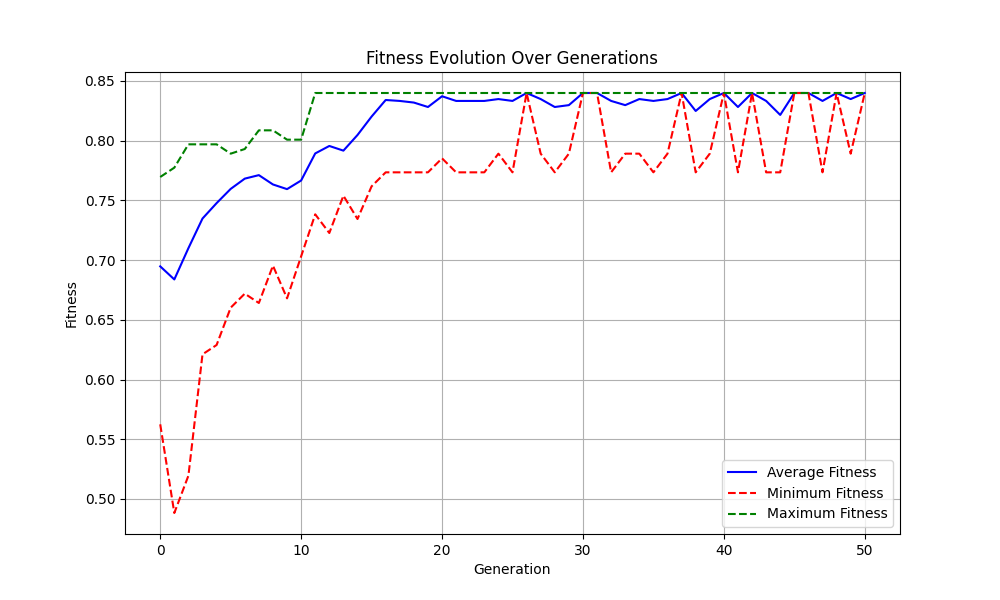
\includegraphics[width=\textwidth]{images/exp_10_fitness_evolution.png}
\caption{Curvas de evolución de la aptitud del experimento 10 con las bandas seleccionadas 220, 113 y 78.}
\label{fig:exp_10_fitness_evolution}
\end{figure}

\begin{figure}[ht]
\centering
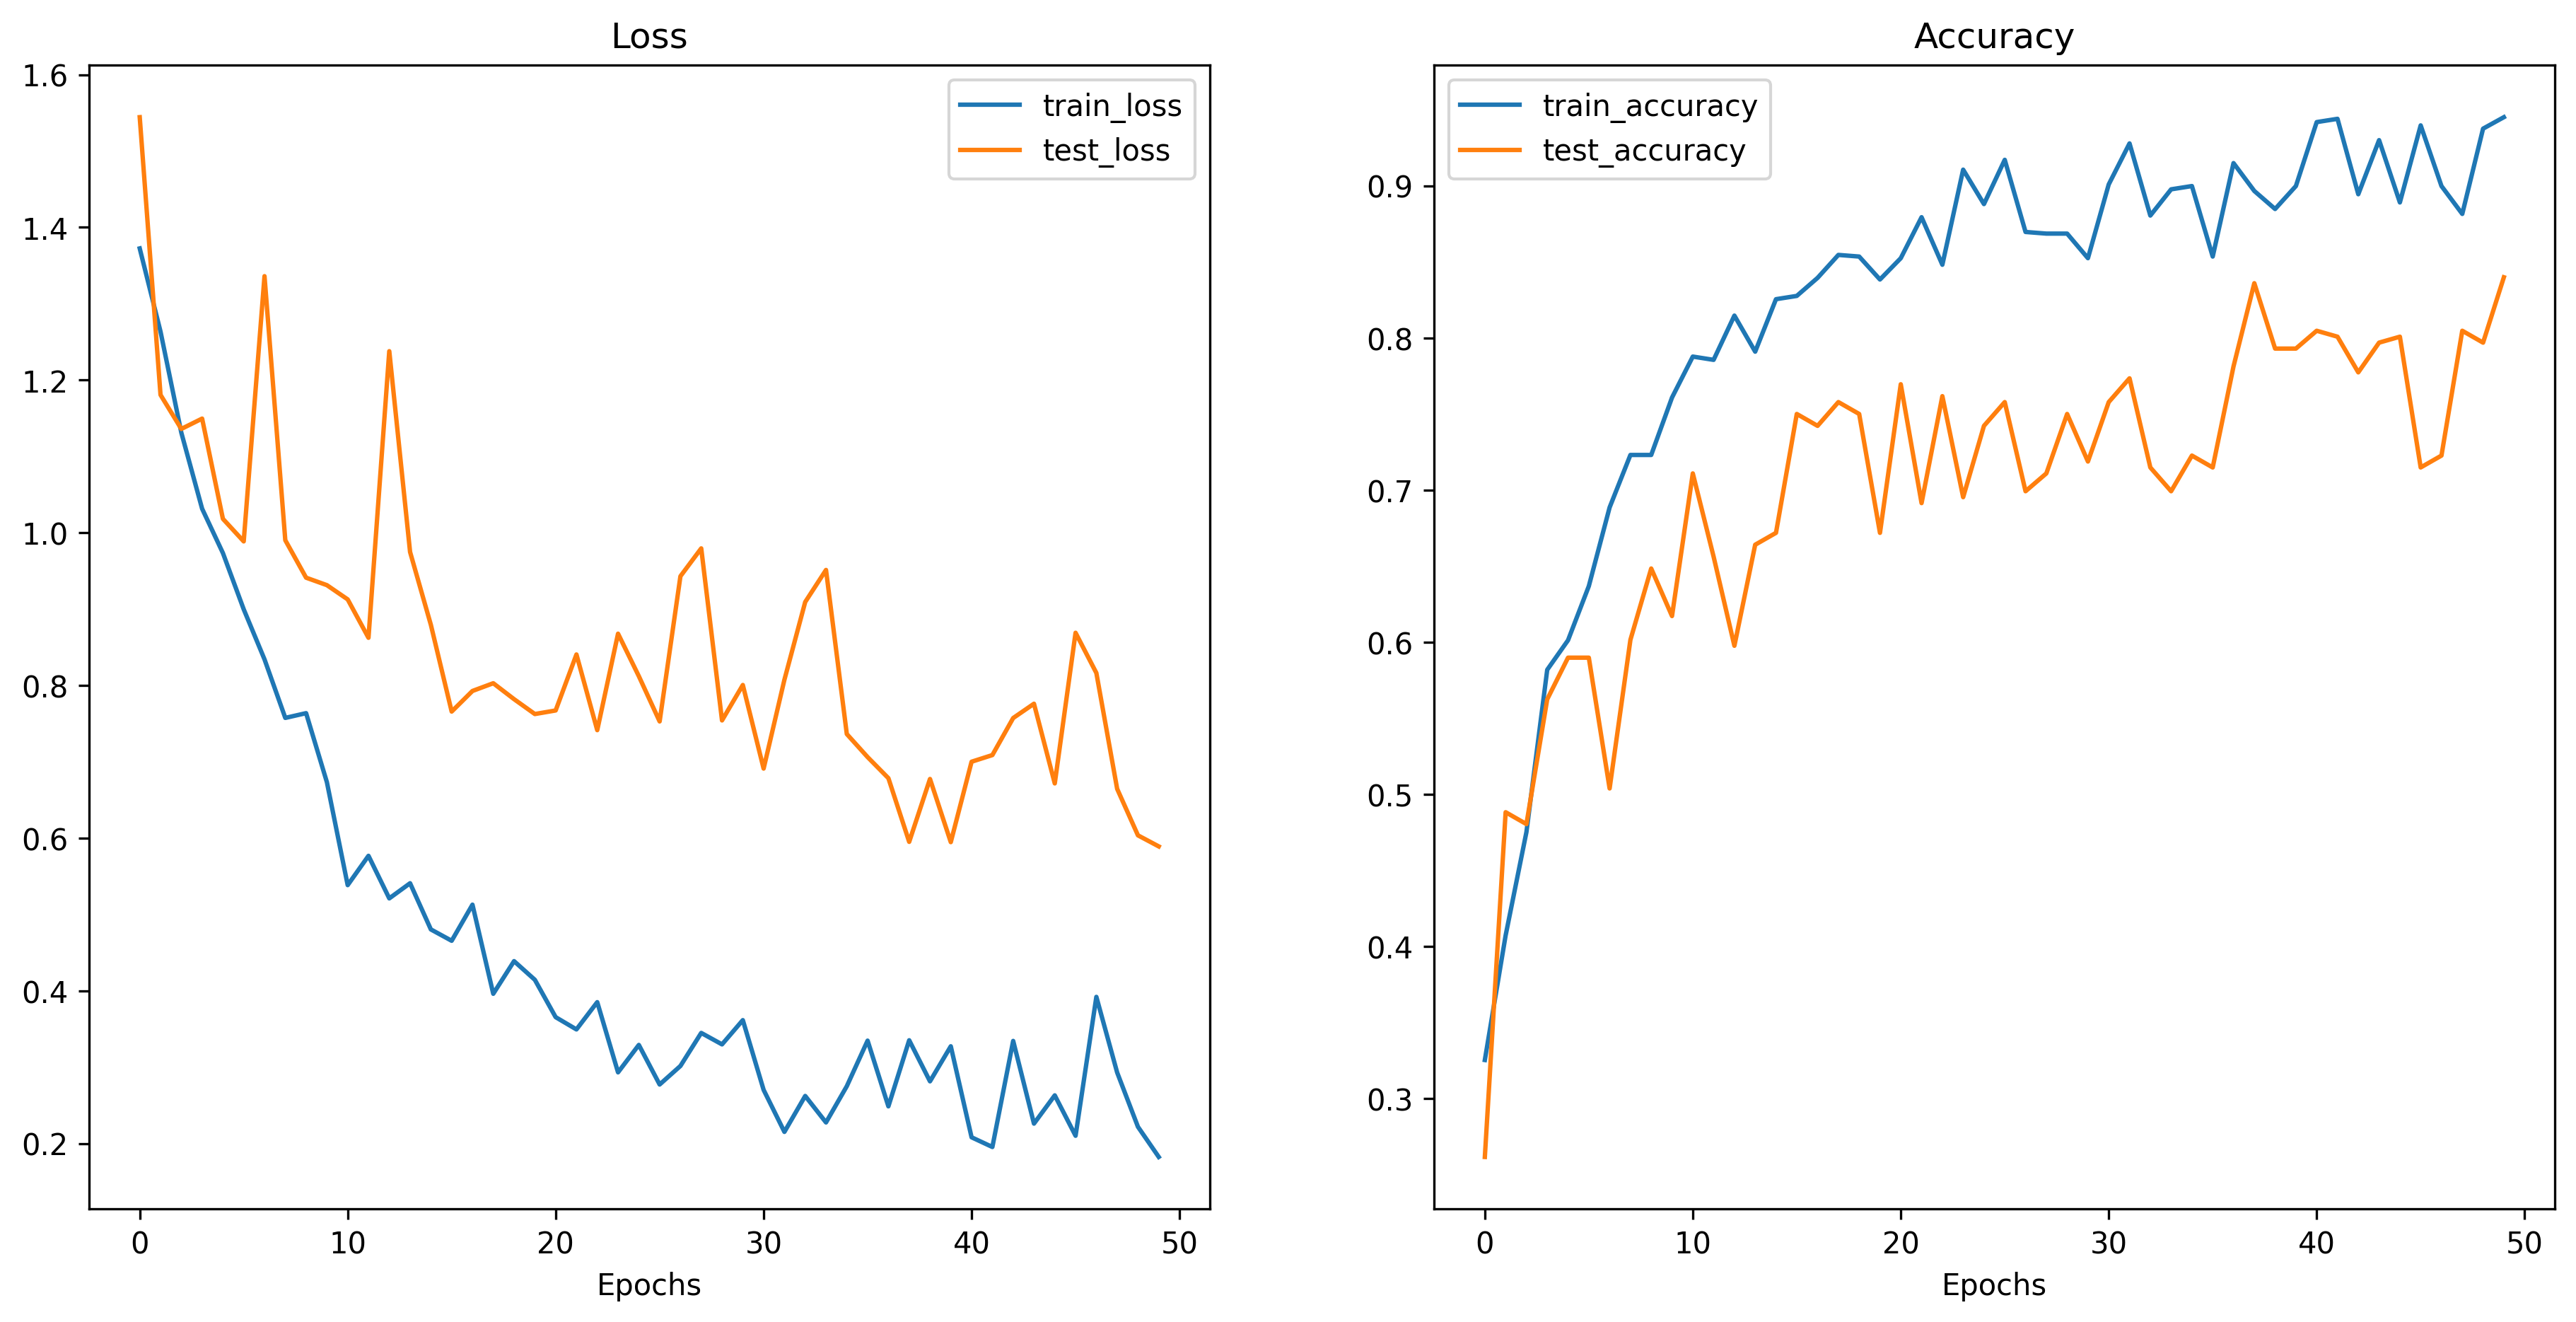
\includegraphics[width=\textwidth]{images/exp_10_cnn_results_220_113_78.png}
\caption{Curvas de precisión y pérdida del experimento 10 con las bandas seleccionadas 220, 113 y 78.}
\label{fig:exp_10_cnn_results_220_113_78}
\end{figure}

\subsection{Desafíos y Observaciones Técnicas}

\section{Análisis Hiperespectral mediante Transformadas Wavelet}

\subsection{Objetivo de la Fase}

La tercera fase del proyecto implementa una metodología alternativa para el análisis de imágenes hiperespectrales mediante la aplicación de transformadas \emph{wavelet} en regiones espacialmente localizadas del higo. Esta aproximación sigue la línea de investigación establecida por Cruz-Carrasco et al. \cite{agriengineering6040225}, quienes demostraron la efectividad del análisis hiperespectral combinado con transformadas \emph{wavelet} para la detección de \emph{Aspergillus flavus} en higos. Sin embargo, mientras que el estudio de referencia realizó el análisis a nivel de píxel individual, esta fase extiende la metodología considerando regiones espaciales más amplias que capturan información contextual y variabilidad espacial local.

\vspace{5mm}

El objetivo principal es explorar la capacidad de las transformadas \emph{wavelet} continuas (CWT) y discretas (DWT) para extraer características espectrales discriminativas a partir de regiones de 32×32 píxeles subdivididas en parches de 4×4 píxeles, permitiendo la clasificación efectiva de diferentes niveles de contaminación por aflatoxinas. Esta aproximación regional, en contraste con el análisis puntual por píxeles, permite capturar patrones espaciales de heterogeneidad espectral que pueden indicar diferentes etapas del desarrollo fúngico y la distribución espacial de la contaminación dentro del tejido del higo.

\vspace{5mm}

Esta aproximación se fundamenta en la hipótesis de que las transformadas \emph{wavelet} pueden capturar información espectral-temporal crítica que métodos tradicionales de procesamiento espectral podrían no detectar. A diferencia de las fases anteriores que operan sobre imágenes \emph{RGB} derivadas o selecciones optimizadas de bandas espectrales, esta metodología procesa directamente la información espectral completa mediante análisis tiempo-frecuencia, preservando tanto las características espectrales como sus variaciones temporales a lo largo del espectro electromagnético.

\subsection{Herramientas y Tecnologías Empleadas}

La implementación de esta fase integra técnicas avanzadas de procesamiento de señales con arquitecturas de aprendizaje profundo especializadas, combinando análisis \emph{wavelet} con redes neuronales convolucionales para la clasificación automatizada de muestras.

\subsubsection{PyWavelets}

\emph{PyWavelets} \cite{lee2019pywavelets} es una biblioteca de Python de código abierto que implementa de manera eficiente y numéricamente estable una amplia gama de transformadas \emph{wavelet}, tanto en su versión discreta como continua. Ofrece soporte para transformadas multiescala, transformadas inversas, y herramientas de análisis como filtrado, compresión y descomposición de señales. La biblioteca incluye múltiples familias de \emph{wavelets} (\emph{Daubechies}, \emph{Morlet}, \emph{Haar}, \emph{Biorthogonal}, entre otras), lo que permite seleccionar la función base más adecuada según la aplicación. En el marco de este proyecto, \emph{PyWavelets} se emplea para transformar firmas espectrales unidimensionales en representaciones tiempo-frecuencia bidimensionales (escalogramas), que capturan de forma localizada tanto las características frecuenciales como su posición en el dominio espectral.

\subsubsection{DenseNet-121}

La arquitectura \emph{DenseNet-121} \cite{huang2018denselyconnectedconvolutionalnetworks} se caracteriza por el uso de conexiones densas entre capas, en las cuales cada capa recibe como entrada no solo la salida de la capa inmediatamente anterior, sino también los mapas de características de todas las capas previas, lo que fomenta una reutilización eficiente de la información aprendida. Esta estrategia de conectividad permite mitigar el problema del desvanecimiento del gradiente, favoreciendo un entrenamiento más estable y profundo, al tiempo que reduce la redundancia de parámetros en comparación con otras arquitecturas tradicionales como \emph{ResNet}, gracias a la mayor eficiencia en el flujo de información. \emph{DenseNet-121}, con sus 121 capas organizadas en bloques densos e intercaladas con capas de transición que controlan la dimensionalidad y la complejidad computacional, logra un equilibrio entre profundidad, capacidad de representación y eficiencia, lo que la convierte en una de las arquitecturas más utilizadas en tareas de clasificación y extracción de características en el dominio del aprendizaje profundo.

\subsection{Flujo de Procesamiento}

El flujo de procesamiento implementa una metodología sistemática que combina extracción espacial de regiones de interés, análisis espectral mediante transformadas \emph{wavelet}, y clasificación mediante aprendizaje profundo.

\subsubsection{1. Extracción de Parches Espectrales}

El proceso comienza con la identificación automática de regiones óptimas de 32×32 píxeles en cada imagen hiperespectral. El algoritmo implementa una estrategia de búsqueda espacial que localiza la región centrada verticalmente y posicionada horizontalmente para minimizar la presencia de píxeles de fondo. Esta selección automatizada garantiza que los parches extraídos contengan exclusivamente información espectral del tejido del higo, eliminando interferencias del fondo de la imagen que podrían introducir ruido en el análisis posterior.

\vspace{5mm}

Una vez identificada la región óptima de 32×32 píxeles, se procede a la subdivisión sistemática en una grilla regular de 64 sub-parches de 4×4 píxeles cada uno. Para cada sub-parche de 4×4 píxeles, se extrae la firma espectral promedio calculando la media aritmética de los valores espectrales a través de las dimensiones espaciales. Este procedimiento de promediado espacial genera 64 firmas espectrales representativas, cada una de 448 bandas espectrales, que capturan la información espectral característica de regiones espacialmente localizadas dentro del higo individual.

\begin{figure}[ht]
\centering
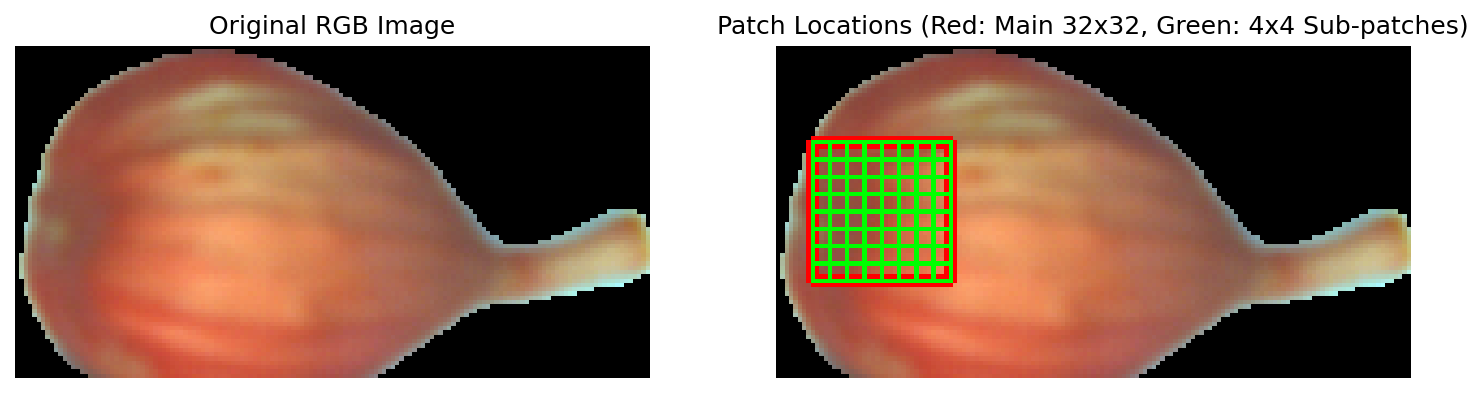
\includegraphics[width=\textwidth]{images/patch_visualization_Fx10_20230717_Riego_C0_2023-07-17_09-02-21_ann0.png}
\caption{Visualización de la región de 32×32 píxeles extraída automáticamente del higo, subdividida en 64 parches de 4×4 píxeles.}
\label{fig:patch_extraction_example}
\end{figure}


Esta metodología de promediado espacial permite reducir el ruido espectral inherente a nivel de píxel individual mientras preserva las características espectrales distintivas de cada región. Al calcular la media espectral de los 16 píxeles (4×4) que componen cada sub-parche, se obtiene una representación espectral más robusta y estable que facilita la identificación de patrones espectrales asociados con diferentes grados de contaminación fúngica.

\begin{figure}[ht]
\centering
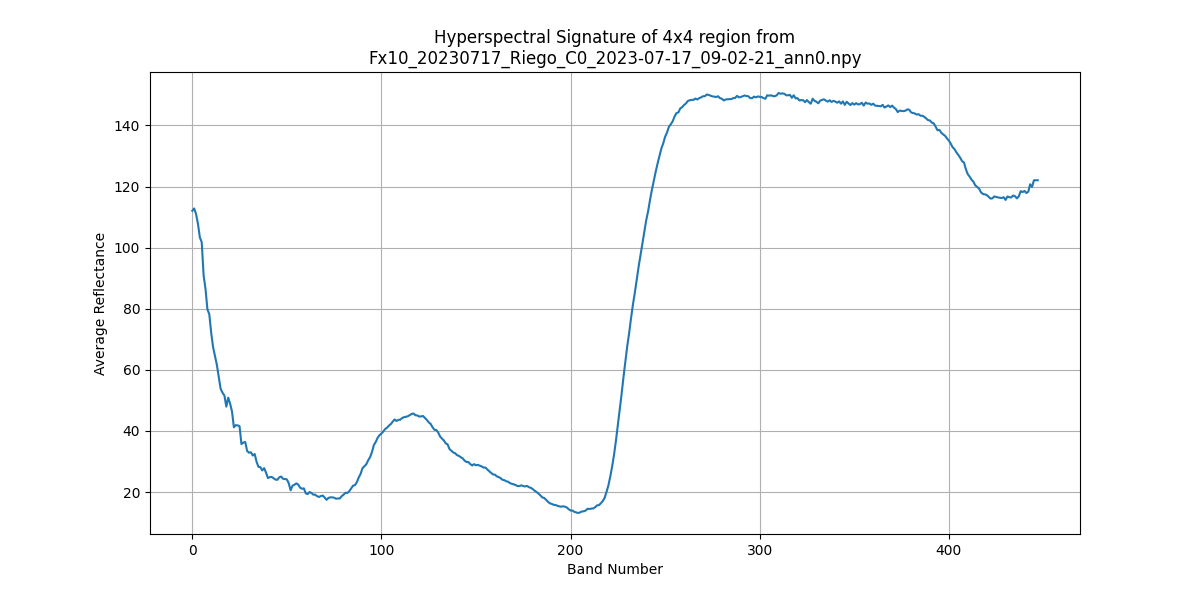
\includegraphics[width=\textwidth]{images/hyperspectral_signature.png}
\caption{Ejemplo de firma espectral promedio extraída de un parche de 4×4 píxeles. La gráfica muestra la reflectancia en función de las 448 bandas espectrales.}
\label{fig:hyperspectral_signature_example}
\end{figure}

\subsubsection{2. Transformada Wavelet Continua}

La transformación espectral utiliza la Transformada Wavelet Continua (\emph{CWT}) con la \emph{wavelet} de \emph{Morlet} como función base. Esta elección se fundamenta en las propiedades óptimas de la \emph{wavelet} de \emph{Morlet} para análisis espectral: proporciona una resolución tiempo-frecuencia balanceada, mantiene fase constante, y exhibe características de localización espectral apropiadas para señales hiperespectrales. La \emph{CWT} se aplica a cada firma espectral de 448 bandas utilizando 64 escalas logarítmicamente distribuidas, generando escalogramas de 64×448 píxeles que representan la distribución tiempo-frecuencia de la información espectral.

\begin{figure}[ht]
\centering
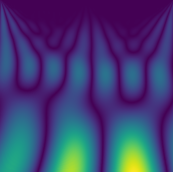
\includegraphics[width=\textwidth]{images/CWT_morl_Fx10_20230717_Riego_C0_2023-07-17_09-02-21_ann0_patch_00.png}
\caption{Ejemplo de escalograma generado por la Transformada Wavelet Continua (\emph{CWT}) utilizando la \emph{wavelet} de \emph{Morlet}.}
\label{fig:cwt_morl_example}
\end{figure}

\vspace{5mm}

Los escalogramas resultantes capturan tanto características espectrales globales como variaciones localizadas en frecuencia, proporcionando una representación rica en información que preserva patrones espectrales discriminativos para la detección de contaminación por aflatoxinas. La selección de 64 escalas permite una cobertura completa del rango espectral mientras mantiene una resolución suficiente para detectar características espectrales finas asociadas con cambios bioquímicos inducidos por el desarrollo fúngico.

\subsubsection{3. Preparación de Datos para CNN}

Los 64 escalogramas generados por cada parche de 32×32 píxeles se organizan como imágenes individuales para el entrenamiento de la red neuronal convolucional. Esta estrategia de aumentado de datos resulta en una expansión significativa del conjunto de datos: cada imagen hiperespectral original genera 64 instancias de entrenamiento, multiplicando efectivamente el tamaño del conjunto de datos disponible para el aprendizaje supervisado.

\vspace{5mm}

Los escalogramas se normalizan utilizando estadísticas estándar de \emph{ImageNet} para aprovechar las ventajas del aprendizaje por transferencia. La organización del conjunto de datos sigue una estructura jerárquica estándar con directorios separados para entrenamiento y prueba, manteniendo la distribución de clases balanceada (\emph{C0}, \emph{C1}, \emph{C2}, \emph{C3}) y preservando la trazabilidad desde las imágenes hiperespectrales originales hasta los escalogramas individuales.

\subsubsection{4. Arquitectura y Entrenamiento de CNN}

La red \emph{DenseNet-121} se adapta específicamente para la clasificación de cuatro clases mediante la modificación de la capa clasificadora final. La arquitectura implementa una cabeza clasificadora personalizada que incluye capas lineales con normalización por lotes, funciones de activación \emph{ReLU}, y regularización mediante \emph{dropout} para prevenir sobreajuste. La configuración final comprende: una capa lineal de 1024 a 128 unidades con \emph{ReLU} y normalización por lotes, seguida de \emph{dropout} (0.4), una segunda capa lineal de 128 a 64 unidades con \emph{ReLU} y \emph{dropout} (0.3), y finalmente una capa de salida de 64 a 4 unidades correspondientes a las clases experimentales.

\vspace{5mm}

El entrenamiento se ejecuta durante 50 épocas utilizando el optimizador \emph{Adam} con tasa de aprendizaje inicial de 0.001 y un planificador \emph{ReduceLROnPlateau} que reduce la tasa de aprendizaje cuando la pérdida de validación se estanca. El modelo utiliza función de pérdida de entropía cruzada y técnicas de aumento de datos que incluyen transformaciones estocásticas apropiadas para imágenes de escalogramas, preservando las características tiempo-frecuencia mientras introducen variabilidad para mejorar la generalización.

\begin{table}[ht]
\centering
\caption{Configuración de la cabeza clasificadora personalizada para \emph{DenseNet-121}.}
\label{tab:custom_layers}
\csvautotabular{tables/custom_layers.csv}
\end{table}

\subsection{Resultados}

La metodología basada en transformadas wavelet demostró una efectividad notable para la clasificación de contaminación por aflatoxinas en muestras de higo. El modelo \emph{DenseNet-121} entrenado alcanzó una precisión de clasificación de \textbf{87.43\%} en el conjunto de prueba, con métricas consistentes a través de las cuatro clases experimentales.

\begin{figure}[ht]
\centering
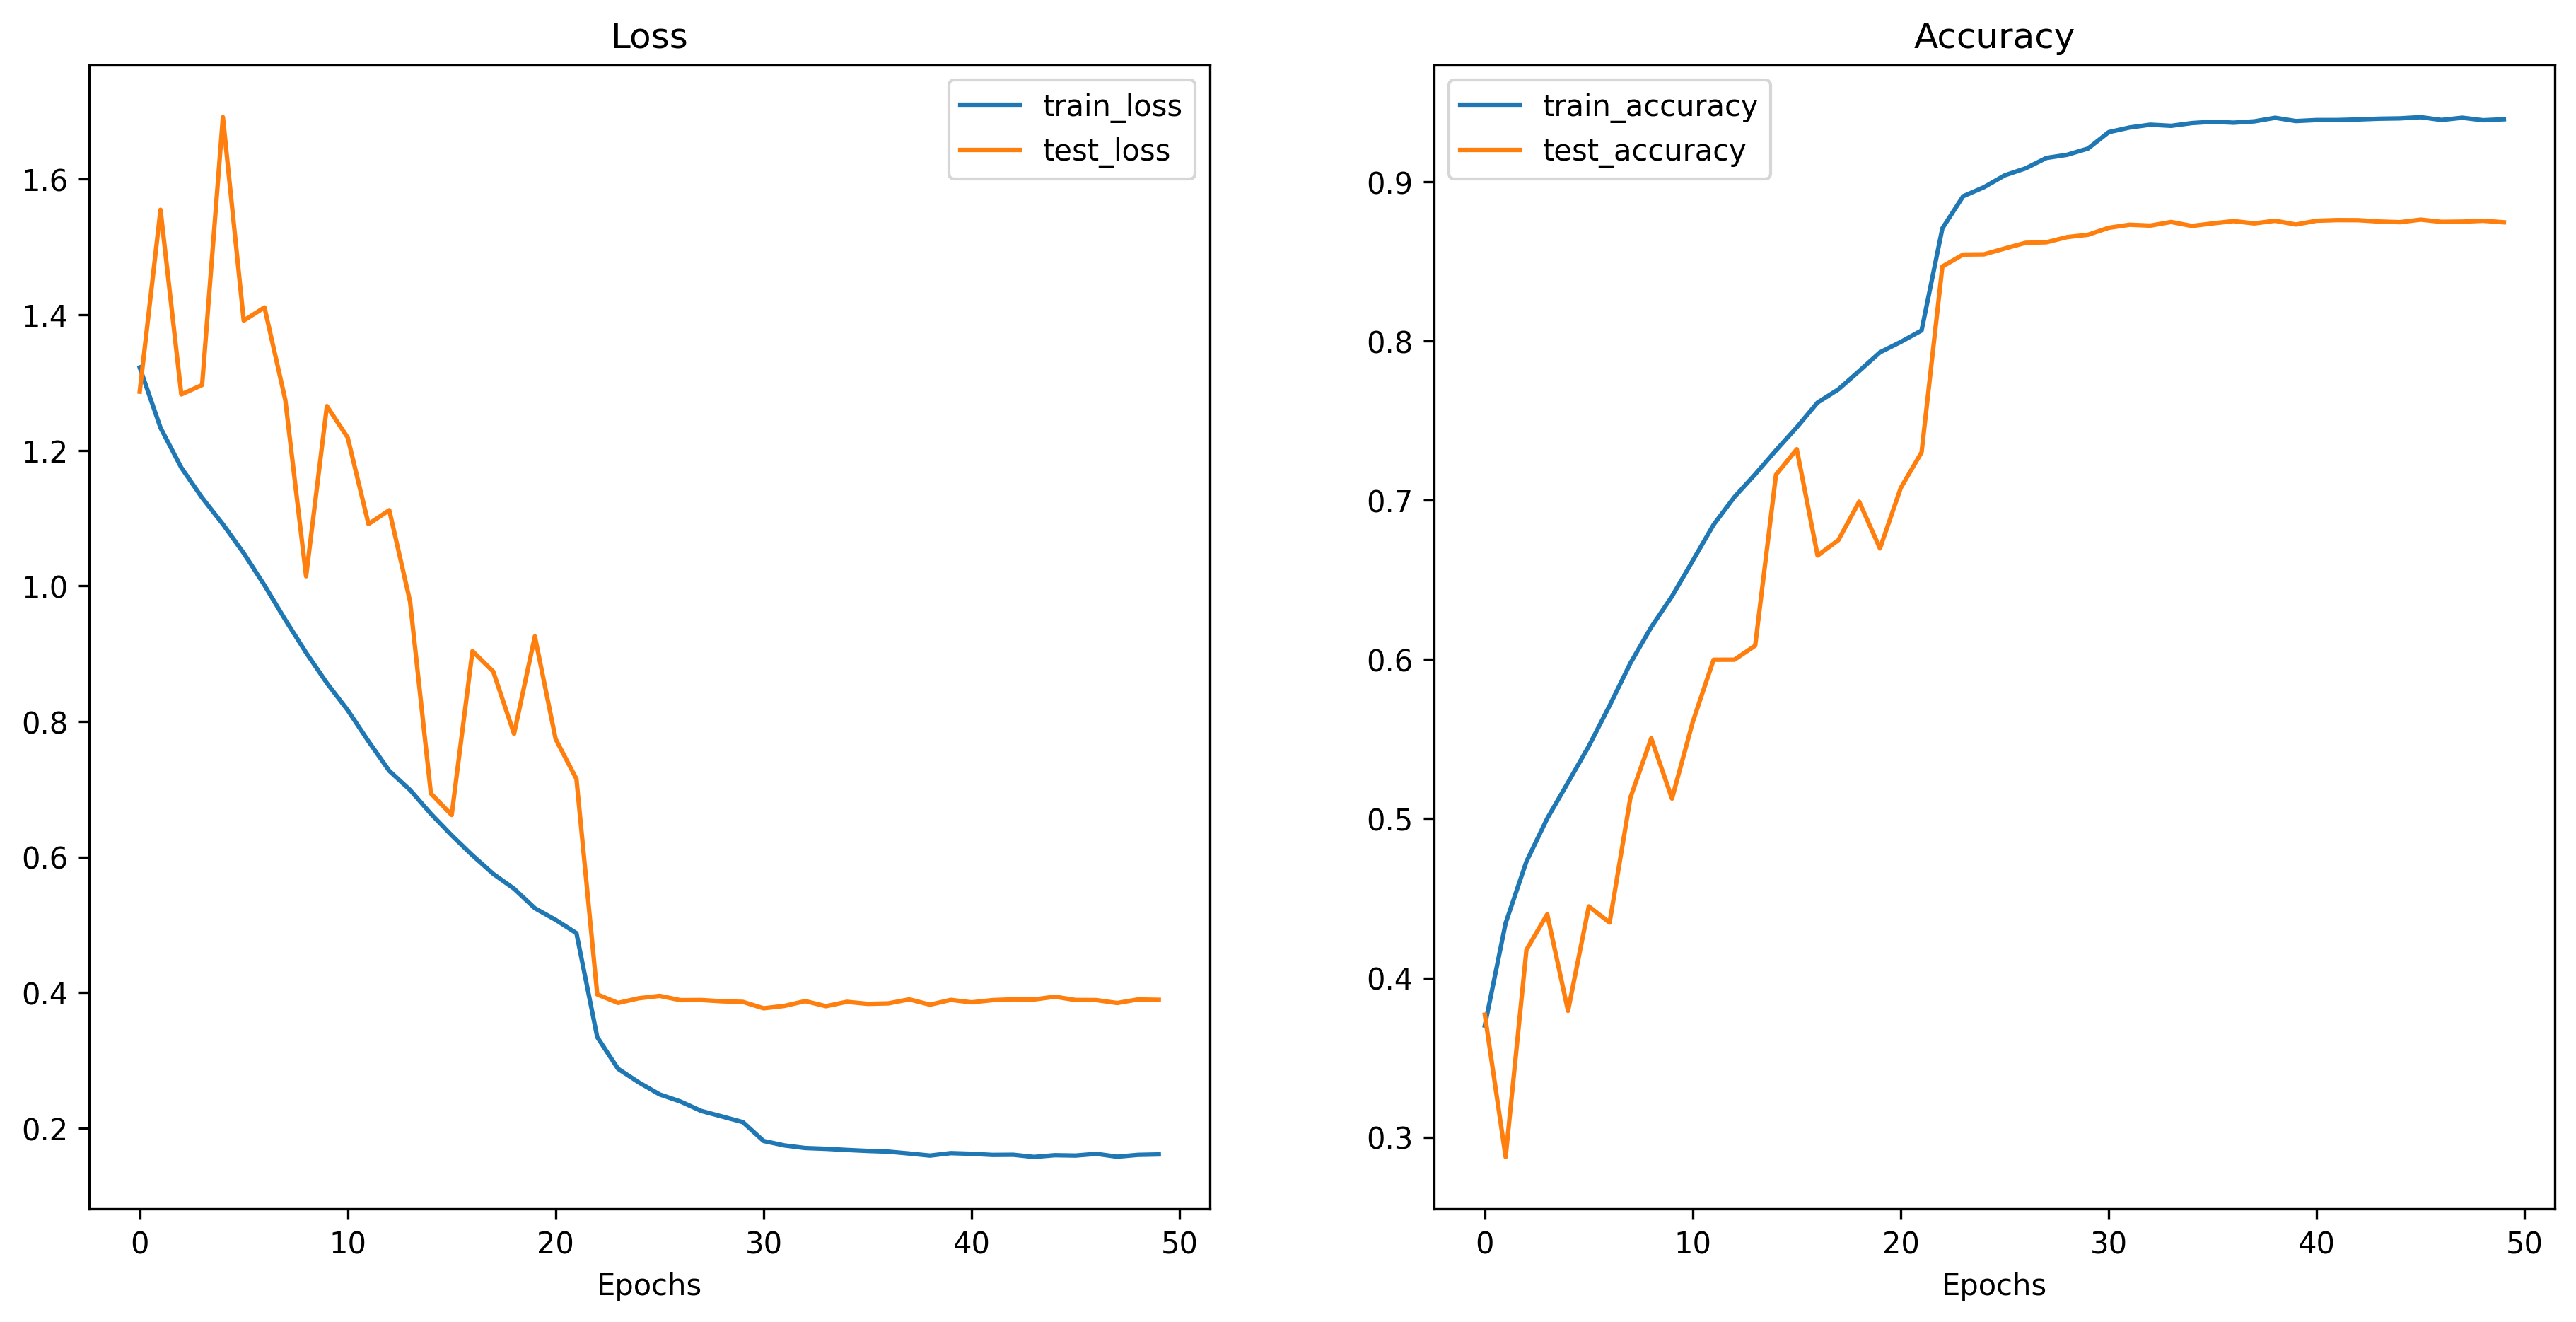
\includegraphics[width=\textwidth]{images/wavelet_training_results.png}
\caption{Curvas de entrenamiento del modelo \emph{DenseNet-121} para clasificación de escalogramas wavelet. Se muestran la evolución de la pérdida y precisión durante 50 épocas de entrenamiento.}
\label{fig:wavelet_training_results}
\end{figure}

\vspace{5mm}

El análisis detallado por clases revela un rendimiento balanceado: \emph{C0} (control sano) alcanzó precisión de 88.92\% y recall de 88.59\%, \emph{C1} (baja contaminación) obtuvo precisión y recall de 88.26\%, \emph{C2} (contaminación media) logró precisión de 85.24\% y recall de 84.49\%, mientras que \emph{C3} (alta contaminación) registró precisión de 87.35\% y recall de 88.43\%. Los puntajes F1 correspondientes fueron 88.76\%, 88.26\%, 84.86\% y 87.89\% respectivamente, indicando un equilibrio efectivo entre precisión y recall en todas las categorías.

\begin{table}[ht]
\centering
\caption{Reporte de clasificación del modelo basado en transformadas wavelet.}
\label{tab:wavelet_report}
\csvautotabular{tables/wavelet_classification_report.csv}
\end{table}

\vspace{5mm}

La matriz de confusión revela patrones de clasificación interpretables: las confusiones más frecuentes ocurren entre clases adyacentes (\emph{C1-C2} y \emph{C2-C3}), reflejando la progresión gradual de la contaminación por aflatoxinas. Específicamente, se observan 190 confusiones entre \emph{C1} y \emph{C2}, y 174 confusiones entre \emph{C2} y \emph{C3}. La clase control (\emph{C0}) muestra la menor tasa de confusión con clases contaminadas, con solo 403 clasificaciones erróneas de un total de 3533 muestras, indicando que la metodología wavelet es efectiva para distinguir muestras sanas de contaminadas.

\begin{table}[ht]
\centering
\caption{Matriz de confusión del modelo basado en transformadas wavelet.}
\label{tab:wavelet_confusion_matrix}
\csvautotabular{tables/wavelet_confusion_matrix.csv}
\end{table}

\vspace{5mm}

El entrenamiento del modelo se completó en 50 épocas, con un tiempo total de entrenamiento de aproximadamente 3.1 horas en una GPU NVIDIA A100. La convergencia del modelo se observa claramente en las curvas de entrenamiento, donde tanto la pérdida como la precisión se estabilizan después de las primeras 20 épocas, indicando un aprendizaje efectivo sin evidencia significativa de sobreajuste.

\subsection{Desafíos y Observaciones Técnicas}

La implementación de la metodología wavelet presentó varios desafíos técnicos que proporcionaron perspectivas valiosas sobre el procesamiento de imágenes hiperespectrales. El primer desafío significativo fue la selección de parámetros óptimos para la CWT, particularmente el número de escalas y su distribución. La experimentación inicial con diferentes configuraciones reveló que 64 escalas logarítmicamente distribuidas proporcionan el mejor equilibrio entre resolución espectral y eficiencia computacional, capturando características espectrales finas sin introducir redundancia excesiva.

\vspace{5mm}

La gestión de memoria constituyó otro aspecto crítico, dado que la generación de escalogramas para el conjunto completo de datos resulta en un volumen significativo de datos procesados. La implementación de procesamiento por lotes y técnicas de liberación explícita de memoria (\texttt{gc.collect()}) después de cada lote de procesamiento permitió manejar eficientemente el flujo de datos sin saturar la memoria disponible. Adicionalmente, se observó que la normalización apropiada de los escalogramas resulta crítica para la convergencia estable del entrenamiento, requiriendo ajustes específicos para accommodar las características únicas de las representaciones tiempo-frecuencia generadas por CWT.

\vspace{5mm}

Un hallazgo técnico importante fue que la metodología wavelet captura información espectral complementaria a las aproximaciones basadas en selección de bandas RGB. Los escalogramas revelan patrones espectrales localizados que no son evidentes en análisis espectrales tradicionales, sugiriendo que las transformadas wavelet proporcionan una perspectiva única para la caracterización de cambios bioquímicos asociados con el desarrollo fúngico y la producción de aflatoxinas en tejidos vegetales.

